\chapter{Pebbles}
\label{chap:410}

This chapter proposes my plan to evaluate Landslide's effectiveness as a debugging aid for students in an educational setting.
This is the second of the three projects I am proposing for this thesis, and is currently ongoing work.
%What remains to be done is detailed in Section~\ref{sec:grading}.

\section{Motivation}

In my MS thesis \cite{landslide}, I solicited students at CMU's Operating Systems Design and Implementation class
(henceforth, ``15-410'')
to volunteer at the end of the P3 project to annotate their kernels and try debugging them with Landslide.
However, the annotation burden undermined Landslide's purpose:
the only students willing to spend free time on manual instrumentation were biased to be those who were already doing well in the class,
and hence least likely to benefit from Landslide's debugging potential.
(Actually, even the best 15-410 students still have concurrency bugs,
but in principle, an educational tool should reach the more struggling students,
the so-called ``middle'' and/or ``bottom'' of the class.)
%
Requiring annotations hurts Landslide's case as a grading tool, as well:
TAs need to understand the kernel to begin with in order to annotate correctly,
and while achieving such understanding they may as well grade it by hand, as before.

Since then, I've extended Landslide to support testing Project 2 (P2) thread libraries (Section~\ref{sec:pebbles}) as well.
Because P2 mandates specific function names for the project's internal APIs
-- most importantly, for the concurrency primitives --
Landslide can automatically annotate arbitrary student implementations with no manual effort required of the user (whether student or TA).
The addition of Quicksand and Iterative Deepening (Chapter~\ref{chap:quicksand}) partly fulfills this purpose,
freeing student attention from the issue of which state spaces to test.
This chapter will detail my further techniques and evaluation which are specific to educational use.

\section{Implementation Details}

Every stateless model checker must make some assumptions about the tested programs' concurrency model \cite{chess}.
However, arbitrary programs may break conventional disciplines of concurrent programs, while still being bug-free.
For example, thread communication via ad-hoc {\tt yield} loops may appear to automated tools as a possible
infinite loop, livelock, or deadlock.
This is especially true of student code,
written by people who are just learning concurrent programming discipline for the first time,
and/or written under the time pressure of a project deadline.
To be an effective tool for struggling students,
a model checker should somehow coax adversarial programs to fit its concurrency model, to effectively test for real bugs,
rather than rejecting them outright on some stylistic or disciplinary grounds.

Fully-automatic instrumentation of student P2s has been no walk in the park.
I have equipped Landslide with several powerful algorithms and heuristics for handling the most common anti-patterns in student submissions.

\begin{itemize}
	\item {\bf Yield-blocking.}
		Landslide recognizes open-coded busy-wait loops used for ad-hoc synchronization,
		and is able to treat threads as blocked (or ``disabled'' in model-checking parlance),
		avoiding getting stuck in an infinitely-long interleaving (or ``cyclic state space'')
		which should never arise during normal execution.
		The heuristically-driven algorithm is as follows:
		\begin{itemize}
			\llitem Whenever a thread performs a {\tt yield}, {\tt xchg}, or other atomic instruction,
				Landslide increments a per-thread counter to track its (supposed) busy-wait loop iterations.
				A thread's counter is reset any time it performs some ``interesting'' activity not likely to appear in a true busy-wait loop:
				any condvar, semaphore, or rwlock invocation (but not mutexes),
				and the beginning or end of any thread library function (create, join, or exit).
				\footnote{Implemented in {\tt check\_user\_yield\_activity} and {\tt check\_user\_xchg} in {\tt user\_sync.c}.}
				The consequence of any this heuristic's inaccuracy is
				that an unusual wait-loop might be classified as an infinite loop bug anyway.
				% TODO: Wow, what happened to KEEP_RUNNING_YIELDING_THREADS?? I swear I had some logic in arbiter.c about that.
			\llitem When a thread's loop counter reaches some heuristic limit (10 for {\tt yield}s, 100 for {\tt xchg}s),
				% Or 20 for xchgs which end up being data-race PPs.
				Landslide speculatively marks the thread blocked (or ``disabled'', in model-checking parlance),
				just as though it had invoked {\tt deschedule}.
				It also retroactively disables that thread at all preceding {\tt yield}s/{\tt xchg}s in that sequence,
				which prevents DPOR from trying to use each as a preemption point,
				and avoids a state space explosion (by a factor of the heuristic yield limit).
				% Well, only the whole state space will explode if this yield-block *always* happens.
				% Otherwise it's (heuristic limit) * (size of subtree) * (number of yield-block occurrences).
				% Tbf, I guess it's very likely for that to be half, or more, of the whole space.
				\footnote{Implemented in {\tt update\_blocked\_transition} in {\tt user\_sync.c}.}
			\llitem When retroactively disabling a thread across all its preceding loop iterations,
				Landslide's state space estimator must account for the ``pruning'' of duplicate subtrees at those (now disabled) preemption points.
				% TODO: Yeah, thinking about this again, I'm pretty sure untag_blocked_branch is deadcode.
				If in any previous thread interleaving, DPOR tagged the now-yield-blocked thread to interleave at another thread's preemption point,
				the estimator would have included that potential subtree in its computation of how much unexplored state space exists.
				Accordingly, in this case Landslide will invert the estimation algorithm,
				including propagating the reduced subtree size all the way to the state space's root.
				\footnote{Implemented in {\tt untag\_blocked\_branch} in {\tt estimate.c}.}
			\llitem Landslide can precisely identify when another thread may trigger the yield-blocking one to fall out of its loop,
				by analyzing the shared memory conflicts involving only accesses performed in the loop.
				At any such memory conflict, Landslide will reenable the yielding thread.
				(If the other thread's access does not fulfill the yielding thread's wait condition,
				the latter will just re-trigger the heuristic and become blocked again.)
				% Hmm.... if two threads are in a deadlock between two ad-hoc loops,
				% and each has some spurious access which kicks the other,
				% it will show up as an infinite loop instead. I guess that's ok?
				\footnote{Implemented in {\tt check\_unblock\_yield\_loop} in {\tt user\_sync.c}.}
		\end{itemize}
		This approach is similar to the Fair-Bounded Search algorithm in \cite{bpor},
		although it avoids a major assumption of the latter (threads {\tt yield} if and only if not making progress),
		and also avoids the need to iteratively deepen the yield bound by instead fixing it as a heuristic constant.
		% Actually, I don't think that's true. Using DPOR to unblock a yield-looping thread at any conflict covers this.
		%The cost of this heuristic is that falsely identifying threads as blocked can lead to unsoundness (...)
	\item {\bf False-positive deadlock avoidance.}
		In contrast to its treatment of data races, Landslide must never report a false-positive {\em bug}.
		If its heuristics falsely identify a thread as blocked, and all other threads are truly blocked,
		waiting on some progress from that thread, Landslide would report a deadlock bug,
		and confuse students horribly.

		The yield-loop heuristic assumes that ``too many'' yields or atomics should not arise during normal, non-looping execution of thread library routines.
		Though extremely rare, this assumption can be violated by an adversarial student submission.
		More often, Landslide can falsely block threads in the special case of {\tt mutex\_test} (see \cite{quicksand}),
		where it uses preemption points within the implementation of {\tt mutex\_lock} itself.
		False deadlocks can also arise from the heuristic blocking of ICB \cite{chess-icb}
		(used in Quicksand's control experiments, Section~\ref{sec:quicksand-eval}).

		When a deadlock arises under conditions where one or more threads are heuristically blocked,
		Landslide attempts to refute it as a false positive by artificially unblocking all heuristically-blocked threads.
		\footnote{If any threads are ICB-blocked, I prioritize waking those before trying to wake any yield-blocked threads.
		% Hmm... I don't remember exactly why.
		Waking all threads at once here can lead to unsoundness.}
		Landslide then repeats this process a heuristic constant number of times (128),
		allowing the program that many chances to make progress before proclaiming deadlock.
		\footnote{Implemented in {\tt try\_avoid\_fp\_deadlock} in {\tt arbiter.c}.}
		Note that this heuristic cannot miss true deadlocks as false negatives:
		if the deadlock is true, each thread will immediately trigger the yield-blocking heuristic again,
		bringing the system back into deadlocked state as many times as necessary to exhaust the heuristic limit.
	\item {\bf Lock hand-off.}
		A common, though discouraged, idiom for implementing thread destruction involves one thread ``handing off'' ownership of a mutex to another.
		That thread will then release the lock with no corresponding acquire in its own execution.
		% In this case, some other thread communication enforces an ordering ... hmm,, pure vs limited hb?
		Although Landslide cannot easily recognize at what point the latter thread's accesses are protected by that lock for the sake of data-race analysis,
		potentially leading to false positive races,
		it must release the lock in its bookkeeping to avoid false {\em negatives} if any later access that should be protected by that lock isn't.
		When releasing a lock, if absent from the current thread's lockset, Landslide searches the locksets of all other existing threads, and releases it there.
		Landslide can instead optionally be configured to treat lock hand-off as a style warning or as an outright bug, as a matter of discipline.
		\footnote{Implemented in {\tt lockset\_remove} in {\tt lockset.c}.}

	% Not really research.
	%\item Other small engineering fixes, such as: recognizing when a system call's access to user memory constitutes a ``communication back-channel'' for user threads that should be considered for DPOR;
\end{itemize}

However, some of the less common offenses are both more difficult to handle algorithmically, and also more worrying from a pedagogical point of view.
%After some collaboration with David Eckhardt (15-410 professor and member of this thesis committee),
For the following cases, I configured Landslide to abort, and warn the student that they must find a better solution before it could test their code (in other words, I promoted these patterns to be treated as bugs).

\begin{itemize}
	\item {\bf Busy-wait loops} containing neither {\tt yield} nor {\tt xchg} (nor any other atomic instruction), such as {\tt while (!other\_thread\_ready) continue;}.
		This blurs the line between anti-pattern and concurrency bug:
		because it does not yield the CPU, a uni-processor machine must wait for the next timer tick (several milliseconds!) before making any progress;
		also, because it does not use atomic instructions, an optimizing compiler may reorder or even delete the loop's accesses.
		%
		Landslide also cannot easily identify it as similar to message-passing,
		appearing indistinguishable
		% not really? there would be dpor conflix, at least
		from a thread-local infinite computation,
		which is of course impossible to judge for halting \cite{entscheidungsproblem}.

		In such a case, Landslide will issue a bug report with the special message:
		{\em I have run a loop in [function name] an alarming number of times.
		This version of Landslide cannot distinguish between this loop being infinite versus merely undesirable.
		Please refer to the ``Synchronization (2)'' lecture.}
	\item {\bf Recursive mutex use} (i.e., locking the same mutex twice in the same thread, then subsequently unlocking it twice).
		While it would not be difficult for Landslide's lock-sets to support recursive locking (using a nesting counter instead of a boolean flag),
		that would assume the corresponding mutex implementation provides the same semantics,
		which is risky business with student code. % ;)
		Furthermore, recursive locking is not an obvious solution to any of P2's challenges;
		far more often, it arises when a student's mutex tries to {\tt malloc} some internal state,
		which itself requires a mutex for safe allocation, which can lead to stack overflow and a crash.

		In such a case, Landslide will issue a bug report with the special message:
		{\em This version of Landslide cannot debug recursive implementations of mutex\_lock.
		Please examine this stack trace and determine for yourself whether it indicates a bug.}
\end{itemize}

\section{Landslide as a Debugging Tool}
\label{sec:studence}

In the Spring 2015, Fall 2015, and Spring 2016 semesters,
I've made Landslide (with Quicksand) available to 15-410 students during the last week of P2.
I introduced stateless model checking in a guest lecture given to the class,
and required students to pass the thread library hurdle \cite{thrlib}
to ensure a minimum of basic functionality necessary to use Landslide.

To analyze its effectiveness as a debugging tool for students,
I configured Landslide to record a snapshot of the inputs and results of each use by the students:
which options were used (test program and time limit),
a snapshot of the student's code, and the result of the test
(completed, timed out, bug found, or ctrl-C'ed).
I manually interpreted the snapshots to determine:
\begin{itemize}
	\item How many unique bugs the student found (discounting multiple runs that produced ``the same'' bug);
	\item How many of those bugs were deterministic versus concurrency bugs (did Landslide find the bug on the first interleaving or did it need to test multiple);
	\item How many of each category of bug the students fixed (determined when a subsequent run of Landslide on the test case failed to find the bug again).
\end{itemize}

{\bf Results -- bugs found.}
Of 90 two-student groups in those 3 semesters, 47 tested their thread libraries with Landslide.
Table~\ref{tab:this-table-sucks-but-it's-the-best-i-got} shows
that Landslide found in total 44 deterministic bugs and 85 concurrency bugs.
It found at least one concurrency bug for 32 groups (68\%),
24 of whom (51\%) were able to fix at least one bug, verifying their update
with a succesful re-run of the same test.
\footnote{The table's data presentation is somewhat confusing:
the dependent columns count the number of {\em groups}, categorized by how many bugs they found, not the raw number of {\em bugs},
instead indicated in the ``Total bugs'' row at the bottom.
So, the number of total bugs is the sum of the products between each cell in that column and its corresponding number of bugs,
e.g., $44 = 27\times0 + 6\times1 + 9\times2 + 2\times3 + 1\times4 + 2\times5$.
%Sorry about that;
I'll try to find a better way to present this data in the thesis.}
I view this as a positive result -- among other statistics, Landslide was able to help the majority of students debug, among those who found concurrency bugs at all -- although it is difficult to control for the amount of time students spent with Landslide that would otherwise have been spent on old-fashioned stress testing.

\begin{table}[h]
	\begin{center}
	\begin{tabular}{r|cc|cc}
	%det bugs found det bugs fixed  races fixed     races found
	& \multicolumn{4}{c}{Number of groups} \\
	Number & \multicolumn{2}{c|}{Deterministic bugs} & \multicolumn{2}{c}{Concurrency bugs} \\
	of bugs & found & fixed & found & fixed \\
	\hline
	0       & 27    & 32    & 15    & 23    \\
	1       & 6     & 5     & 7     & 11    \\
	2       & 9     & 6     & 12    & 8     \\
	3       & 2     & 1     & 7     & 2     \\
	4       & 1     & 1     & 3     & 1     \\
	5       & 2     & 2     & 2     & 1     \\
	11      &       &       & 1     & 1     \\
	\hline
	%Total groups
	%       & 47    & 47    & 47    & 47    \\
	Total bugs
	        & 44    & 34    & 85    & 53    \\
	\end{tabular}
	\end{center}
	\caption{Summary of how many bugs were found and/or fixed by how many groups.
	Each column counts how many groups found/fixed the number of bugs in each row;
	for instance, two groups found 5 concurrency bugs, one of which fixed all 5.}
	\label{tab:this-table-sucks-but-it's-the-best-i-got}
\end{table}

{\bf Results -- impact on grades.}
Next, I investigated the impact Landslide ultimately had on students' performance.
I collected the ultimate P2 and P3 grades from the last 6 semesters, forming three categories:
students from the past 3 semesters who volunteered to use Landslide,
students from those semesters who opted out,
and students from the other 3 semesters, for whom Landslide was not available at all.
I hoped to measure a correlation between use of Landslide and ultimate P2 grades,
which would show that it helps students submit more correct P2s,
and/or a correlation with ultimate P3 grades,
which would (tentatively) show that it teaches better ways of thinking that students retain for future projects (i.e., measuring actual learning).

Unfortunately, this turned out to be a negative result, as shown in Figure~\ref{fig:grade-distribution}.
The distribution of Landslide users' ultimate grades is indistinguishable from that of students for whom Landslide was unavailable.
While there was a 3\% increase in P2 grades between opt-out-ers and Landslide users, it's prone to selection bias:
perhaps those who opted out of Landslide were already the worst of the class who simply didn't have any free time for it.
The distribution of P3 grades is indistinguishable as well.
In the thesis, I will discuss possible factors contributing to this failure, and how they might be controlled for in future work.
%although I am not planning to run any further experiments in the limited time I have.

\begin{figure}[h]
	\begin{center}
	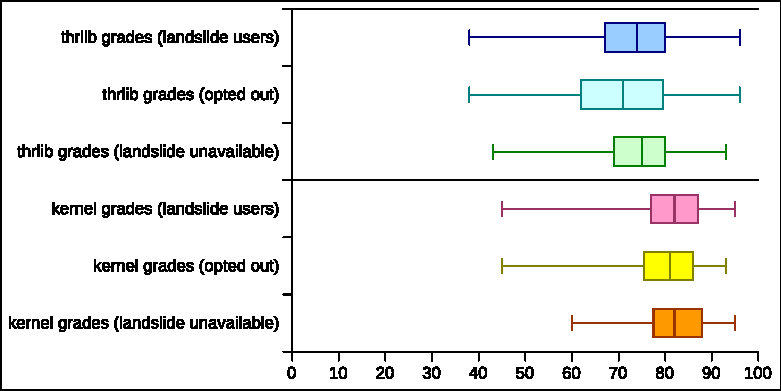
\includegraphics[width=0.85\textwidth]{p2-p3-distribution.pdf}
	\end{center}
	\caption{Distribution of P2 (thrlib) and P3 (kernel) grades among students who did or didn't use Landslide.}
	\label{fig:grade-distribution}
\end{figure}


{\bf Future work.}
One evaluation question remains which I will answer in the thesis:
what is the accuracy of Landslide's automation heuristics?
In other words, were false-positive infinite loops or deadlocks ever reported
where Landslide failed to recognize an ad-hoc synchronization?
(I expect a near 100\% success rate,
having tuned the heuristics by hand on an (independent) set of P2 submissions already.)
%
%\section{Landslide as a Grading Tool}
%\label{sec:grading}
%
%Beginning in 2017, I will recruit 15-410 Teaching Assistants (TAs) for my user study rather than students.
%The modified user study will evaluate Landslide as a grading tool,
%alternative to the ``Fritz'' stress-testing infrastructure which 15-410 currently employs,
%and possibly substituting as well for the human process of reading student code looking for concurrency bugs by hand.
%The intent is not for Landslide to ultimately replace 15-410's manual grading process,
%but rather to demonstrate that comparably-rigorous grading could be deployed automatedly at other schools wishing to adopt the 15-410 curriculum.
%
%I will pursue the following evaluation questions:
%
%\begin{itemize}
%	\item Provided appropriate test cases, can Landslide find the most common ``deep'' concurrency bugs in student submissions?
%	\item How does Landslide's bug-finding compare to that of Fritz, the class's stress tester?
%	\item How does Landslide's bug-finding compare to that of TAs grading by hand?
%\end{itemize}
%
Finally, I will conclude this chapter in the thesis by discussing how future work could adapt Pebbles's interface to support fully-automatic model checking without compromising the educational value of P3.
